% Compile with XeLaTeX (Devanagari needs fontspec + HarfBuzz shaping):
%   tectonic main.tex      or      latexmk -xelatex main.tex      (Overleaf: set compiler to XeLaTeX)
\documentclass[11pt]{article}

\usepackage[a4paper,margin=1in]{geometry}
\usepackage{fontspec}
\usepackage{amsmath,amssymb}
\usepackage{booktabs,array,tabularx,multirow}
\usepackage{xcolor}
\usepackage{tikz}
\usetikzlibrary{arrows.meta,positioning,calc,fit}
\usepackage{pgfplots}
\pgfplotsset{compat=1.18}
\usepackage[font=small,labelfont=bf]{caption}
\usepackage[shortlabels]{enumitem}
\usepackage[round]{natbib}
\usepackage{microtype}
\usepackage[colorlinks,linkcolor=accent,citecolor=accent,urlcolor=accent]{hyperref}

% Bundled Noto Sans Devanagari (SIL OFL), so the source compiles anywhere.
\newfontfamily\devfont{NotoSansDevanagari}[
  Path=fonts/, Extension=.ttf, UprightFont=*-Regular, BoldFont=*-Bold,
  Script=Devanagari, Scale=MatchLowercase]
\newcommand{\hi}[1]{{\devfont #1}}
\newcommand{\vsp}{\textvisiblespace}
\newcommand{\nohyph}{\hyphenpenalty=10000\exhyphenpenalty=10000\relax}
\newcommand{\hd}[1]{\begin{tabular}[b]{@{}c@{}}#1\end{tabular}}

\definecolor{accent}{HTML}{2B6CB0}
\definecolor{muted}{HTML}{A8A79E}
\definecolor{mutedlight}{HTML}{D6D5CE}
\definecolor{quiet}{HTML}{5F5E58}

\setlist{itemsep=2pt,topsep=4pt}

\title{Cheaper Hindi Without Forgetting:\\Boundary-Aligned Self-Distillation for Tokenizer Extension}
\author{
  Aaryan Regmi\\\texttt{regmi\_aaryan@srmap.edu.in}
  \and Yajnesh Ande\\\texttt{yajnesh\_ande@srmap.edu.in}
  \and Sheldon Castelino\\\texttt{castelino\_theodore@srmap.edu.in}
}
\date{SRM University--AP, Andhra Pradesh, India\\[4pt]November 2026}

\begin{document}
\maketitle

\begin{abstract}
Appending 256 Hindi merges to Qwen3-4B-Instruct-2507 cuts Hindi prompt tokens by 34\%. Naive adaptation of the new tokens, however, breaks the model: Hindi reading falls and copying collapses (0/112 on a template probe). The copy failure traces to a handful of new tokens: the model emits a spaceless native character in place of a space-prefixed merged token, or drops a vowel sign.
Continued-BPE merges nest inside native tokens, so every expanded-token boundary is also a native one, and the frozen native model is an exact teacher at those boundaries. We use this for \emph{boundary-aligned self-distillation}: multi-layer hidden-state and next-token alignment at shared boundaries, plus training on the native model's own responses, with 256 new rows and rank-16 LoRA on 1.5M tokens.
On a sealed TEST set (2,588 items, evaluated once) the distilled model keeps the full 34\% token saving. Hindi Belebele comes within 1.9 points of the native model (95\% CI $[-4.5, +0.6]$), English Belebele is exactly unchanged, and the model follows the answer format more reliably. Finding the answer span in Hindi QA ($-5.0$ points) and character-exact copying of varied text remain worse.
An ablation shows the alignment terms matter: training on the teacher's responses alone leaves 24 of 112 template copies broken, and adding boundary alignment fixes all of them. We also show that strict benchmark scores overstate such recoveries, because they reward format and brevity, and we report a separate content score for every task.
\end{abstract}

%======================================================================
\section{Introduction}

Hindi pays a large, tokenizer-specific token tax \citep{petrov2023unfairness,ahia2023cost}, and the tax turns into real compute under long-context, batched serving. On 1,012 aligned FLORES+ sentences \citep{nllb2022}, Qwen2.5's tokenizer uses $4.49\times$ $[4.43, 4.54]$ as many tokens for Hindi as for English. A BLOOM tokenizer trained with more Indic text removes 92\% of that excess, so the cost belongs to the tokenizer, not the language.

On short single prompts the latency penalty is only $1.00$--$1.03\times$. At 256-token contexts with batch size 4, prefill latency reaches $5.1\times$ for Hindi and $7.5\times$ for Tamil. KV-cache memory scales exactly with token count (Appendix~\ref{app:tax}).

Extending a pretrained model's vocabulary is the direct fix, and on the tokenizer side it works. With 256 continued-BPE merges \citep{sennrich2016bpe}, Qwen3-4B-Instruct-2507 \citep{yang2025qwen3} needs 35.8\% fewer tokens for held-out Hindi and 34.1\% fewer for chat-rendered Belebele prompts, with English unchanged. The model side is the problem: after 1M tokens of standard adaptation, Hindi reading drops and literal copying fails.

\paragraph{Contributions.}
\begin{enumerate}
  \item \textbf{A token-level diagnosis of the failure (\S\ref{sec:diagnosis}).} At 128 new tokens, the copy failure sits in 4 of the 22 new tokens the probe needs. At 4,096 new tokens the failure becomes romanization and digit collapse.
  \item \textbf{Boundary-aligned self-distillation (\S\ref{sec:method}).} The expanded tokenization is a strict coarsening of the native one, so the frozen native model is an exact teacher at every expanded boundary. No cross-tokenizer approximation is needed.
  \item \textbf{A sealed-TEST evaluation that separates content from format (\S\ref{sec:results}).} At the full token saving, Hindi reading comes within 1.9 points of native and English is unchanged. Extraction and character-exact copying remain measurably worse.
\end{enumerate}

%======================================================================
\section{Setup}
\label{sec:setup}

One pinned model, one ranked merge list, and paired comparisons against the unmodified model on the same items.

\paragraph{Model.} \texttt{Qwen/Qwen3-4B-Instruct-2507}, revision \texttt{cdbee75f}, BF16, with the original weights frozen. New token IDs start after the full 151,936-row matrix, so every native ID, including chat special tokens, keeps its ID. Disabling the new rows and adapters reproduces native logits bit-identically on an H100.

\paragraph{Vocabulary.} Continued BPE was fitted on a document-disjoint split of Sangraha Verified Hindi \citep{khan2024indicllmsuite}. The 128-, 256-, 512- and 4,096-token vocabularies are prefixes of one ranked merge list, and each passed one million round-trip checks. We use 256, the smallest size that clears a 25\% prompt-token reduction on every Hindi task (Table~\ref{tab:vocab}).

\begin{table}[h]
\centering\small
\caption{Token change against the native tokenizer, by vocabulary extension size.}
\label{tab:vocab}
\begin{tabular}{rcccc}
\toprule
New tokens & Hindi corpus & Belebele-hi prompts & Exact-detail prompts & English corpus \\
\midrule
128   & $-30.0\%$ & $-28.4\%$ & $-22.8\%$ & $-0.08\%$ \\
\textbf{256} & $\mathbf{-35.8\%}$ & $\mathbf{-34.1\%}$ & $\mathbf{-26.8\%}$ & $\mathbf{-0.09\%}$ \\
4,096 & $-45.9\%$ & $-44.5\%$ & $-41.2\%$ & --- \\
\bottomrule
\end{tabular}
\end{table}

\paragraph{Evaluation.} All tasks are scored on greedy generation from Qwen chat-rendered prompts. Token counts are measured on those rendered prompts.
\begin{itemize}
  \item \textbf{DEV (822 items):} Belebele \citep{bandarkar2024belebele} hin\_Deva (176) and eng\_Latn (184); XQuAD-hi \citep{artetxe2020xquad} (192); the prior 112-item exact-detail copy probe; 8 mixed-script copy items; and a new 150-item diverse Hindi copy probe (one sentence each from 150 held-out documents, under 3 instruction templates).
  \item \textbf{TEST (2,588 items):} Belebele-hi (724), Belebele-en (716), XQuAD-hi (998), and a fresh 150-item copy probe from tokenizer-TEST documents.
\end{itemize}

\paragraph{Protocol.} Benchmark membership was frozen by passage hash before any training. The candidate was selected on DEV and its checkpoint hash sealed before TEST was opened. Both the native control and the candidate were evaluated on TEST exactly once (Figure~\ref{fig:protocol}).

\begin{figure}[h]
\centering
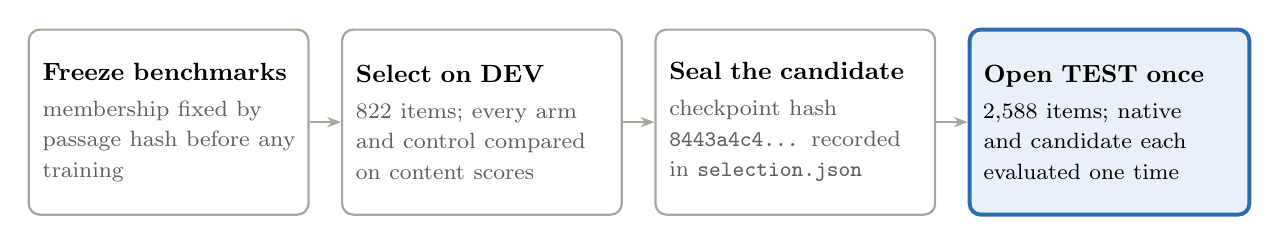
\begin{tikzpicture}[
  stage/.style={draw=muted, rounded corners=4pt, line width=0.8pt, text width=3.2cm, minimum height=2.35cm, align=left, inner sep=5pt, font=\small\nohyph},
  keystage/.style={stage, draw=accent, fill=accent!10, line width=1.4pt},
  arr/.style={-{Stealth[length=5pt]}, draw=muted, line width=0.8pt}]
\node[stage] (a) {\textbf{Freeze benchmarks}\\[2pt]{\color{quiet}\footnotesize membership fixed by passage hash before any training}};
\node[stage, right=0.4cm of a] (b) {\textbf{Select on DEV}\\[2pt]{\color{quiet}\footnotesize 822 items; every arm and control compared on content scores}};
\node[stage, right=0.4cm of b] (c) {\textbf{Seal the candidate}\\[2pt]{\color{quiet}\footnotesize checkpoint hash \texttt{8443a4c4\ldots} recorded in \texttt{selection.json}}};
\node[keystage, right=0.4cm of c] (d) {\textbf{Open TEST once}\\[2pt]{\footnotesize 2,588 items; native and candidate each evaluated one time}};
\draw[arr] (a) -- (b); \draw[arr] (b) -- (c); \draw[arr] (c) -- (d);
\end{tikzpicture}
\caption{Evaluation protocol. The candidate was chosen on DEV and its checkpoint hash sealed before TEST was opened. The ablations in \S\ref{sec:ablations} ran on DEV only; TEST was never reused.}
\label{fig:protocol}
\end{figure}

\paragraph{Statistics.} Paired differences against the native model use 95\% passage-clustered bootstrap intervals (10,000 resamples) and exact McNemar tests.

\paragraph{Scoring.} Every task gets a strict score and a content score:
\begin{itemize}
  \item \textbf{Belebele:} strict = the output is exactly the letter; content = the first answer letter.
  \item \textbf{XQuAD:} strict = exact match and token F1; content = whether the gold span appears in the output.
  \item \textbf{Copy probes:} strict = exact output; content = whether the reference appears in the output.
\end{itemize}

%======================================================================
\section{Why naive extension fails}
\label{sec:diagnosis}

The copy collapse after naive extension comes from a few specific new tokens, and its character changes with vocabulary size. All evidence comes from saved DEV predictions. We re-decoded every emitted ID sequence through the merge decomposition and the native tokenizer, and the result matches the stored text exactly. These are genuine model outputs, not detokenization artifacts.

\paragraph{The legacy copy probe is narrower than it looks.} All 112 exact-detail references share one sentence template once digits are masked; only 39 references are distinct. The strict metric also penalizes the \texttt{[1]} label that the prompt invites: the native model scores 28/112 strict but contains the reference in 112/112. We therefore added the 150-item diverse probe and report containment alongside strict scores.

\paragraph{At 128 new tokens, four rows break copying.} The template needs 22 distinct new tokens, and the model emits 18 of them at ${\geq}90\%$ of the required rate. The four failures are in Table~\ref{tab:fail}.

\begin{table}[h]
\centering\small
\caption{The four new tokens (of 22 needed) that the naive 128-row model fails to emit. \vsp{} marks a leading space.}
\label{tab:fail}
\begin{tabular}{llrrl}
\toprule
New token & Native byte pieces & Needed & Emitted & Model emits instead \\
\midrule
\vsp\hi{फ}   & \texttt{Ġà¤} + \texttt{«} & 112 & 3   & \hi{फ}, space lost \\
\vsp\hi{ज}   & \texttt{Ġà¤} + \texttt{ľ} & 336 & 96  & \hi{ज}, space lost \\
\hi{ै।}      & \texttt{à¥} + \texttt{Ī} + \texttt{।} & 112 & 32 & \hi{।}, vowel sign lost \\
\hi{ीं}      & \texttt{à¥Ģ} + \texttt{à¤Ĥ} & 224 & 115 & \hi{ी}, nasal mark lost \\
\bottomrule
\end{tabular}
\end{table}

Every item contains these tokens, so every item fails, even though mean character F1 is 0.988. Restricting decoding to native output IDs does not restore reading (101/176 either way), so the input side is implicated too.

\paragraph{At 4,096 new tokens the failure changes kind.} The dominant errors become romanization (\hi{कविता ने}~$\to$~\texttt{kavita ne}, \hi{है।}~$\to$~\texttt{hai.}), digit collapse (\hi{२०२६}~$\to$~\hi{२०००}), and word substitution. Mean character F1 falls to 0.463. Small extensions fail at particular rows; large ones lose the script.

\paragraph{Reading loss is real at 256 rows.} Against native, the naive 256-row model loses 18 Belebele-hi items and gains 6 (strict, $p=0.02$), and loses 31 and gains 10 on XQuAD span containment ($p=0.001$).

%======================================================================
\section{Method: boundary-aligned self-distillation}
\label{sec:method}

The expanded model is trained to reproduce the frozen native model at every boundary the two tokenizations share. It also learns to emit the canonical merged tokens.

\paragraph{Exact alignment.} Every new token decomposes into a fixed sequence of native tokens, and merges apply only inside pre-tokens. The expanded tokenization $s$ of a text therefore expands exactly to its native tokenization $n$. Each student position $j$ maps to the native position $e(j)$ where its last piece ends (Figure~\ref{fig:method}). We verified this on 400 chat-rendered training texts with no exceptions, special tokens included. The teacher is the same network with new rows and adapters switched off, which is bit-exact to the original. No second model copy and no cross-tokenizer marginalization are needed.

\begin{figure}[t]
\centering
\begin{tikzpicture}[x=1.6cm, y=1cm,
  tok/.style={draw=muted, rounded corners=3pt, line width=0.8pt, minimum height=0.72cm, inner sep=0pt, font=\large},
  newtok/.style={tok, draw=accent, fill=accent!12, line width=1.3pt},
  bnd/.style={draw=accent, line width=1pt, dash pattern=on 3pt off 2pt}]
% shared boundaries (native token indices)
\foreach \k in {0,3,5,6,8,9} \draw[bnd] (\k,0.62) -- (\k,-2.32);
% native row (teacher)
\node[anchor=south west, font=\small, inner sep=0] at (0,0.78) {\textbf{Teacher:} the same network with new rows and LoRA off, native tokenizer (9 tokens)};
\foreach \k/\t in {0/{\vsp\hi{न}\ldots}, 1/{\ldots\hi{न}}, 2/{\hi{ह}}, 3/{\hi{◌ी}}, 4/{\hi{◌ं}}, 5/{\vsp\hi{ह}}, 6/{\hi{◌ु}}, 7/{\hi{आ}}, 8/{\hi{।}}}
  \node[tok, minimum width=1.46cm] at (\k+0.5,0) {\t};
% expanded row (student)
\node[newtok, minimum width=3*1.6cm-0.14cm] at (1.5,-1.7) {\vsp\hi{नह}};
\node[newtok, minimum width=2*1.6cm-0.14cm] at (4.0,-1.7) {\hi{◌ीं}};
\node[tok,    minimum width=1.46cm]          at (5.5,-1.7) {\vsp\hi{ह}};
\node[newtok, minimum width=2*1.6cm-0.14cm] at (7.0,-1.7) {\hi{◌ुआ}};
\node[tok,    minimum width=1.46cm]          at (8.5,-1.7) {\hi{।}};
\node[anchor=north west, font=\small, inner sep=0] at (0,-2.48) {\textbf{Student:} same network + 256 new rows + rank-16 LoRA, expanded tokenizer (5 tokens)};
% legend
\node[newtok, minimum width=0.35cm, minimum height=0.3cm] at (0.12,-3.3) {};
\node[anchor=west, font=\footnotesize, text=quiet] at (0.25,-3.3) {new merged token};
\draw[bnd] (2.2,-3.3) -- (2.55,-3.3);
\node[anchor=west, font=\footnotesize, text=quiet] at (2.6,-3.3) {shared boundary: 6 of the 10 native boundaries};
\node[anchor=west, font=\footnotesize, text=quiet, inner sep=0] at (0,-3.8) {\vsp{} = leading space;\ \ \ldots\hi{न} = one character split across two byte-level native tokens};
\end{tikzpicture}
\caption{Boundary alignment on a real phrase, \hi{नहीं हुआ।} (``did not happen''), under the native and 256-row tokenizers. The three new tokens each cover two or three native tokens, so all six expanded boundaries are native boundaries too. At those points the teacher's hidden states and next-token distribution are exact targets for the student.}
\label{fig:method}
\end{figure}

\paragraph{Data.} No gold labels and no benchmark text are used.
\begin{itemize}
  \item \textbf{Prompts:} 3,000 instruction prompts built from the adaptation split (2,400 Hindi, 600 English) across six tasks: summarize, list facts, extract the $k$-th sentence, translate, state the topic, and cloze multiple choice. Every template is worded differently from every evaluation template.
  \item \textbf{Raw text:} 1,000 segments.
  \item \textbf{Responses:} the native model answered every prompt greedily. Responses that hit the length limit, 53\% of them, are kept as exact prefixes and trained without an end-of-turn token. Hindi's token cost is why so many hit the limit.
\end{itemize}

\paragraph{Loss.} For each sequence, with $\hat h$ an L2-normalized hidden state, $L=\{9,18,27\}$ of 36 layers, $W_0$ the frozen native output head, and $\lambda_h=\lambda_k=1$:
\begin{equation}
\begin{split}
\mathcal{L} = {}& \mathrm{CE}\big(s_{\text{resp}}\big)
 + \lambda_h \Big[ \tfrac{1}{|L|} \sum_{l \in L} \big\| \hat h^{S}_{l,j} - \hat h^{T}_{l,e(j)} \big\|^2
 + \big\| \hat h^{S}_{\text{final},j} - \hat h^{T}_{\text{final},e(j)} \big\|^2 \Big] \\
 &+ \lambda_k \, \mathrm{KL}\big( p_T(\cdot \mid e(j)) \,\big\|\, \mathrm{softmax}(W_0 \hat h^{S}_{\text{final},j}) \big)
\end{split}
\end{equation}
The three terms do different jobs:
\begin{itemize}
  \item \textbf{Cross-entropy} is computed on the teacher's responses (on all tokens for raw text), in the expanded tokenization with the full extended head. It is what teaches the canonical merged tokens such as \vsp\hi{ज}, the exact failure in \S\ref{sec:diagnosis}.
  \item \textbf{The hidden-state term} averages over all shared boundaries, prompt included. That covers the input side, which \S\ref{sec:diagnosis} implicates in the reading loss.
  \item \textbf{The KL term} \citep{hinton2015distilling} uses 128 random boundaries per sequence.
\end{itemize}

\paragraph{Parameters and budget.} 256 untied new input and output rows, initialized as the mean of their native pieces, plus rank-16 LoRA \citep{hu2022lora} on all attention and MLP projections: 34.3M trainable parameters. Learning rates are $5\times10^{-4}$ for the rows and $10^{-4}$ for LoRA (AdamW, accumulation 8). Training ran for one pass over 1.5M native-token-equivalents (2,061 sequences) in 44 minutes on a shared H100, peaking at 8.4\,GiB. Native mode stays bit-exact because the adapters and rows can be switched off.

%======================================================================
\section{Results}
\label{sec:results}

On sealed TEST, the distilled model keeps the 34\% Hindi token saving. It reads Hindi within 1.9 points of the native model and leaves English unchanged. Span extraction and character-exact copying remain worse.

\subsection{Sealed TEST (evaluated once)}

\begin{table}[h]
\centering\small
\caption{Sealed TEST, content scores. Differences are ours minus native, in points, with 95\% passage-clustered bootstrap CIs.}
\label{tab:test}
\setlength{\tabcolsep}{4pt}
\begin{tabular}{llrrlrr}
\toprule
Task (items) & Content score & Native & Ours & \hd{Ours $-$ native\\{}[95\% CI]} & \hd{McNemar\\$p$} & \hd{Prompt\\tokens} \\
\midrule
Belebele-hi (724)  & first answer letter & 505 & 491 & $-1.9$ $[-4.5, +0.6]$ & 0.18 & $-34.1\%$ \\
Belebele-en (716)  & first answer letter & 640 & 640 & $0.0$ $[-0.6, +0.6]$ & 1.0 & 0\% \\
XQuAD-hi (998)     & gold span in output & 757 & 707 & $-5.0$ $[-7.5, -2.5]$ & $<$0.001 & $-35.2\%$ \\
Diverse copy (150) & reference in output & 121 & 92 & $-19.3$ $[-27.3, -11.3]$ & $<$0.001 & $-31.7\%$ \\
\bottomrule
\end{tabular}
\end{table}

Batch-16 and batch-1 greedy decoding agreed on 32/32 checked items for both models. The candidate checkpoint (\texttt{8443a4c4\ldots}) matches the selection sealed on DEV.

Hindi reading is not significantly different from native, but the interval's lower end ($-4.5$) means non-inferiority within 2 points is not established. English is unchanged to within $\pm0.6$ points.

\subsection{Strict scores overstate recovery}
\label{sec:strict}

On strict scores, the distilled model \emph{beats} native on every Hindi task: Belebele-hi 491 vs.\ 459 ($+4.4$ $[+1.4, +7.5]$); XQuAD exact match 206 vs.\ 82 and token F1 0.477 vs.\ 0.353; diverse copy exact 90 vs.\ 84. These gains are format and brevity, not comprehension (Figure~\ref{fig:strict}):
\begin{itemize}
  \item \textbf{Belebele:} the distilled model answers with a bare letter on 724/724 Hindi items, against 650/724 for native, which sometimes appends the option text.
  \item \textbf{XQuAD:} its answers are shorter (DEV median 43 vs.\ 71 characters), which raises exact match and F1 even though the gold span appears less often.
\end{itemize}

\begin{figure}[t]
\centering
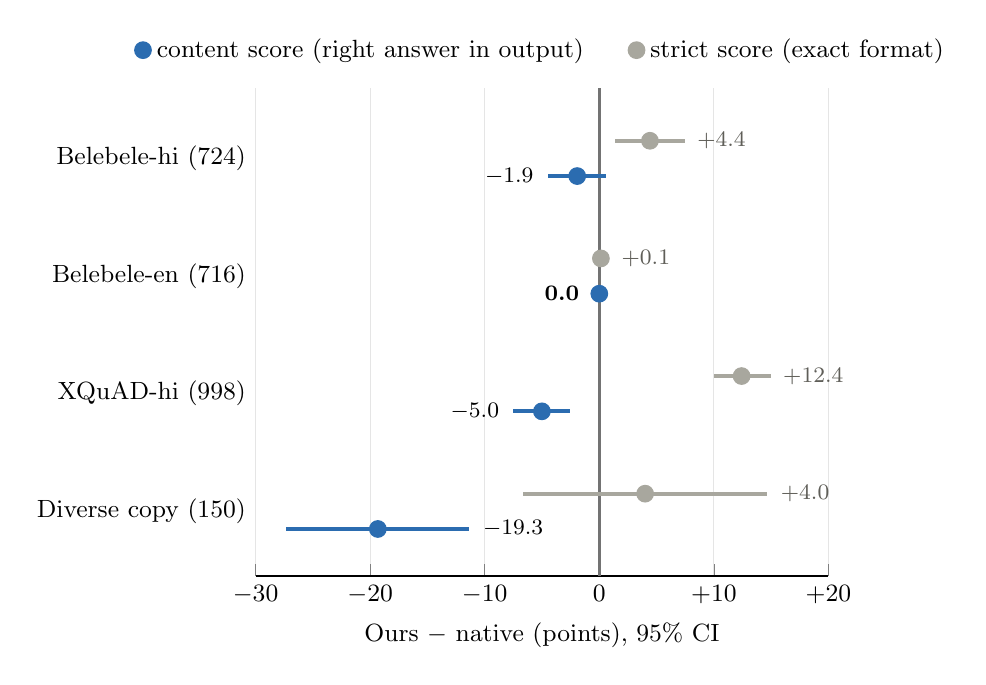
\begin{tikzpicture}
\begin{axis}[
  scale only axis, width=0.6\linewidth, height=6.2cm,
  xmin=-30, xmax=20, ymin=0.45, ymax=4.6, clip=false,
  xtick={-30,-20,-10,0,10,20},
  xticklabels={$-30$,$-20$,$-10$,0,$+10$,$+20$},
  ytick={1,2,3,4},
  yticklabels={{Diverse copy (150)},{XQuAD-hi (998)},{Belebele-en (716)},{Belebele-hi (724)}},
  yticklabel style={font=\small},
  xlabel={Ours $-$ native (points), 95\% CI},
  xlabel style={font=\small}, ticklabel style={font=\small},
  xmajorgrids, major grid style={draw=black!10},
  axis y line*=left, axis x line*=bottom, y axis line style={draw=none}, ytick style={draw=none},
  legend style={at={(0.5,1.03)}, anchor=south, draw=none, font=\small, legend columns=2, /tikz/every even column/.append style={column sep=14pt}},
  error bars/error bar style={line width=1.4pt},
  error bars/error mark=none,
]
\draw[black!55, line width=0.9pt] (axis cs:0,0.45) -- (axis cs:0,4.6);
\addplot+[only marks, mark=*, mark size=3pt, color=accent, mark options={fill=accent},
  error bars/.cd, x dir=both, x explicit]
  coordinates {(-1.93,3.85) += (2.48,0) -= (2.56,0)
               (0.00,2.85) += (0.56,0) -= (0.56,0)
               (-5.01,1.85) += (2.47,0) -= (2.52,0)
               (-19.33,0.85) += (8.00,0) -= (8.00,0)};
\addlegendentry{content score (right answer in output)}
\addplot+[only marks, mark=*, mark size=3pt, color=muted, mark options={fill=muted},
  error bars/.cd, x dir=both, x explicit]
  coordinates {(4.42,4.15) += (3.04,0) -= (3.02,0)
               (0.14,3.15) += (0.68,0) -= (0.56,0)
               (12.42,2.15) += (2.53,0) -= (2.39,0)
               (4.00,1.15) += (10.67,0) -= (10.67,0)};
\addlegendentry{strict score (exact format)}
\node[font=\footnotesize\bfseries, anchor=east] at (axis cs:-4.9,3.85) {$-1.9$};
\node[font=\footnotesize\bfseries, anchor=east] at (axis cs:-0.9,2.85) {0.0};
\node[font=\footnotesize\bfseries, anchor=east] at (axis cs:-7.9,1.85) {$-5.0$};
\node[font=\footnotesize\bfseries, anchor=west] at (axis cs:-11.0,0.85) {$-19.3$};
\node[font=\footnotesize, text=quiet, anchor=west] at (axis cs:7.7,4.15) {$+4.4$};
\node[font=\footnotesize, text=quiet, anchor=west] at (axis cs:1.1,3.15) {$+0.1$};
\node[font=\footnotesize, text=quiet, anchor=west] at (axis cs:15.2,2.15) {$+12.4$};
\node[font=\footnotesize, text=quiet, anchor=west] at (axis cs:15.0,1.15) {$+4.0$};
\end{axis}
\end{tikzpicture}
\caption{The same sealed-TEST predictions under two scorings. Every strict gain on Hindi turns into a loss once the answer is checked for content rather than format.}
\label{fig:strict}
\end{figure}

This matters beyond this paper. Vocabulary-adaptation results scored only by strict letter match or EM/F1 can report recovery that is really a change of output style.

\subsection{Against the baselines (DEV)}
\label{sec:baselines}

\begin{table}[h]
\centering\small
\caption{DEV, 822 items, content scores (items correct). Bold marks the notable failure of each baseline. $^a$Trained on 1M tokens of raw text (80\% Hindi, 20\% English by bytes). Naive expansion trains only the 256 new rows plus a rank-64 adapter on them, with the model body frozen; native-tokenizer LoRA adds no tokens.}
\label{tab:dev}
\setlength{\tabcolsep}{4pt}
\begin{tabular}{lrrrrrr}
\toprule
Model & \hd{Belebele\\-hi} & \hd{Belebele\\-en} & \hd{XQuAD-hi\\span} & \hd{Exact-detail\\copy} & \hd{Diverse\\copy} & \hd{Hindi prompt\\tokens} \\
\midrule
Native (frozen)                       & 119 & 173 & 137 & 112 & 121 & baseline \\
Native-tokenizer LoRA$^a$ & 122 & \textbf{163} & 129 & 111 & 138 & 0\% \\
Naive 256-row expansion$^a$ & 114 & 173 & 116 & \textbf{0} & \textbf{34} & $-34\%$ \\
\textbf{Ours} (1.5M distillation) & 118 & 173 & 125 & 112 & 89 & $-34\%$ \\
\bottomrule
\end{tabular}
\end{table}

Against naive expansion, distillation recovers about 80\% of the Belebele-hi loss, 43\% of the XQuAD loss and 63\% of the diverse-copy loss, and it fully restores exact-detail copying (Table~\ref{tab:dev}, Figure~\ref{fig:recovery}).

Ordinary adaptation with the native tokenizer is not a free alternative. It gains slightly on Hindi but costs English 5.4 points $[-8.8, -2.7]$. Distillation leaves English exactly unchanged on DEV and TEST, because the adapter learns the identity wherever the two tokenizations coincide.

\begin{figure}[t]
\centering
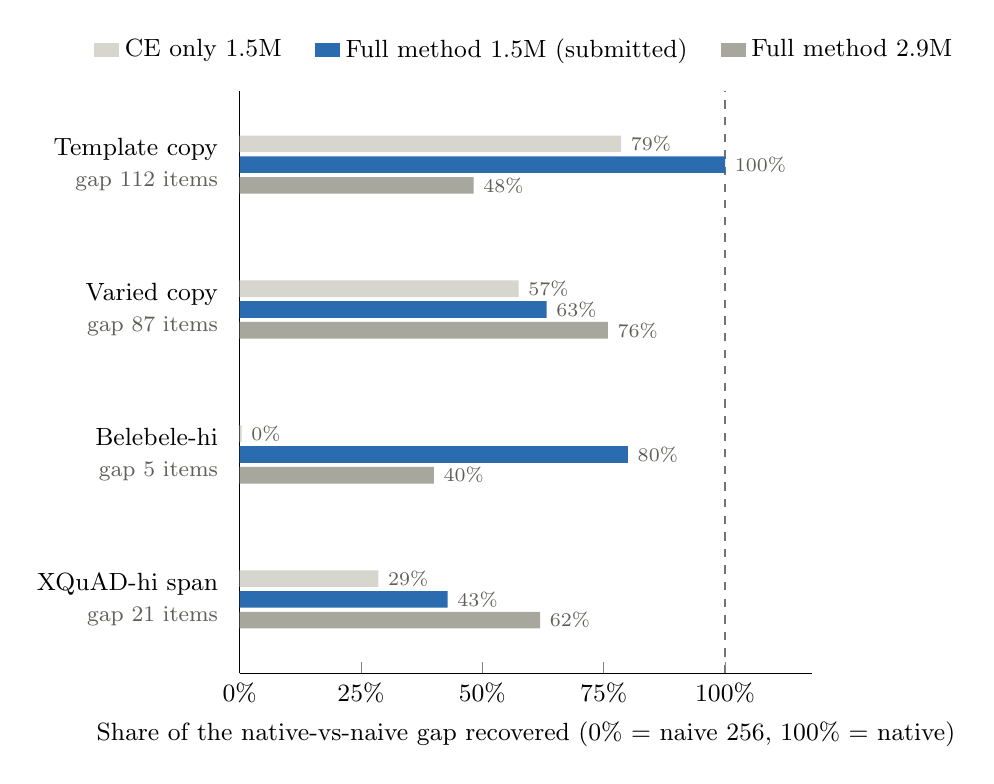
\begin{tikzpicture}
\begin{axis}[
  xbar=1.5pt, bar width=6pt,
  scale only axis, width=0.6\linewidth, height=7.4cm,
  xmin=0, xmax=118,
  xtick={0,25,50,75,100},
  xticklabels={0\%,25\%,50\%,75\%,100\%},
  extra x ticks={100}, extra x tick labels={},
  extra x tick style={grid=major, major grid style={draw=black!55, dashed, line width=0.8pt}},
  symbolic y coords={XQuAD-hi span,Belebele-hi,Varied copy,Template copy},
  ytick=data,
  yticklabels={{XQuAD-hi span\\{\footnotesize\color{quiet}gap 21 items}},{Belebele-hi\\{\footnotesize\color{quiet}gap 5 items}},{Varied copy\\{\footnotesize\color{quiet}gap 87 items}},{Template copy\\{\footnotesize\color{quiet}gap 112 items}}},
  yticklabel style={align=right, font=\small},
  enlarge y limits=0.17,
  axis x line*=bottom, axis y line*=left, ytick style={draw=none},
  xlabel={Share of the native-vs-naive gap recovered (0\% = naive 256, 100\% = native)},
  xlabel style={font=\small}, ticklabel style={font=\small},
  nodes near coords={\pgfmathprintnumber[fixed,precision=0]{\pgfplotspointmeta}\%},
  nodes near coords style={font=\scriptsize, color=quiet},
  every node near coord/.append style={anchor=west},
  point meta=explicit symbolic,
  reverse legend,
  legend image code/.code={\fill[#1] (0cm,-0.09cm) rectangle (0.32cm,0.09cm);},
  legend style={at={(0.5,1.03)}, anchor=south, draw=none, font=\small, legend columns=3, /tikz/every even column/.append style={column sep=10pt}},
]
\addplot[draw=none, fill=muted] coordinates
  {(61.90,XQuAD-hi span) [61.90] (40,Belebele-hi) [40] (75.86,Varied copy) [75.86] (48.21,Template copy) [48.21]};
\addplot[draw=none, fill=accent] coordinates
  {(42.86,XQuAD-hi span) [42.86] (80,Belebele-hi) [80] (63.22,Varied copy) [63.22] (100,Template copy) [100]};
\addplot[draw=none, fill=mutedlight] coordinates
  {(28.57,XQuAD-hi span) [28.57] (0.4,Belebele-hi) [0] (57.47,Varied copy) [57.47] (78.57,Template copy) [78.57]};
\legend{Full method 2.9M, Full method 1.5M (submitted), CE only 1.5M}
\end{axis}
\end{tikzpicture}
\caption{How much of the naive-extension loss each variant recovers on DEV (content scores); the two ablations are described in \S\ref{sec:ablations}. Only the submitted model fully recovers template copying, and no variant fully recovers QA or varied copying. Belebele-hi's gap is only 5 items, so its percentages are noisy.}
\label{fig:recovery}
\end{figure}

\subsection{What is still lost}

The remaining copy errors are normalizations of the source, not the collapse of \S\ref{sec:diagnosis}. On TEST, 20 of the 58 misses are a single change: a sentence-final ``\texttt{.}'' written as the Hindi danda \hi{।}. Most of the rest are spelling standardizations (\hi{शुरु}~$\to$~\hi{शुरू}), agreement changes (\hi{थे}~$\to$~\hi{था}), and a few dropped vowel signs (\hi{कहा}~$\to$~\hi{कह}).

Mean character F1 is 0.995 against native's 0.851. The distilled model reproduces the content closely, but does not preserve nonstandard orthography. That rules it out, for now, where exact strings matter: IDs, names, legal text.

\subsection{Ablations (DEV)}
\label{sec:ablations}

\paragraph{Is boundary alignment needed?} We trained the same model on the teacher's responses with cross-entropy only (no hidden-state or KL terms), at the same 1.5M-token budget and seed. Table~\ref{tab:ce} pairs it with the full method on DEV, on content scores. ``Wins'' counts items only that model got right.

\begin{table}[h]
\centering\small
\caption{Cross-entropy only vs.\ the full method (DEV, content scores).}
\label{tab:ce}
\setlength{\tabcolsep}{4pt}
\begin{tabular}{lrrrrrr}
\toprule
Task (items) & Native & \hd{Naive\\256} & \hd{CE\\only} & \hd{Full\\method} & \hd{Wins\\full / CE} & \hd{$p$\\(McNemar)} \\
\midrule
Exact-detail copy, contained (112) & 112 & 0 & 88 & \textbf{112} & 24 / 0 & $<$0.001 \\
Diverse copy, contained (150)      & 121 & 34 & 84 & 89 & 15 / 10 & 0.42 \\
Belebele-hi, first letter (176)    & 119 & 114 & 114 & 118 & 12 / 8 & 0.50 \\
XQuAD span contained (192)         & 137 & 116 & 122 & 125 & 16 / 13 & 0.71 \\
Belebele-en, first letter (184)    & 173 & 173 & 172 & 173 & 1 / 0 & 1.00 \\
\bottomrule
\end{tabular}
\end{table}

\begin{itemize}
  \item \textbf{Alignment fixes the copy failure.} Cross-entropy alone leaves 24 of 112 template copies broken. The full method gets all 24 right and loses none. This is the failure the diagnosis traced to a few new tokens. Matching the native model's states at shared boundaries removes it; imitating its outputs does not.
  \item \textbf{Elsewhere the alignment terms help a little, but not significantly.} On Hindi reading, cross-entropy alone scores the same as naive expansion (114), and the full method recovers to 118. With 176 items this is suggestive, not significant. Diverse copy and XQuAD move in the same direction, within noise.
  \item \textbf{Strict scores mislead again.} Cross-entropy alone scores higher on strict XQuAD exact match (53 vs.\ 38 of 192) because its answers are shorter, while it contains the answer less often (122 vs.\ 125).
\end{itemize}

\paragraph{Does more data close the copy gap?} We ran the same method over all 4,000 adaptation prompts: 2.9M native tokens, about twice the main run (Table~\ref{tab:3m}).

\begin{table}[h]
\centering\small
\caption{Main run (1.5M tokens) vs.\ twice the data (2.9M tokens), DEV content scores.}
\label{tab:3m}
\setlength{\tabcolsep}{4pt}
\begin{tabular}{lrrrrr}
\toprule
Task (items) & Native & \hd{1.5M\\(main)} & 2.9M & \hd{Wins\\1.5M / 2.9M} & \hd{$p$\\(McNemar)} \\
\midrule
Template copy, contained (112)   & 112 & \textbf{112} & 54 & 58 / 0 & $<$0.001 \\
Varied copy, contained (150)     & 121 & 89 & 100 & 17 / 28 & 0.14 \\
Belebele-hi, first letter (176)  & 119 & 118 & 116 & 11 / 9 & 0.82 \\
XQuAD span contained (192)       & 137 & 125 & 129 & 10 / 14 & 0.54 \\
Belebele-en, first letter (184)  & 173 & 173 & 173 & 0 / 0 & 1.00 \\
\bottomrule
\end{tabular}
\end{table}

\begin{itemize}
  \item \textbf{More data moves the copy gap rather than closing it.} Varied copying and Hindi QA improve (100 vs.\ 89 and 129 vs.\ 125), though not significantly.
  \item \textbf{Template copying breaks on a single substitution.} All 58 new misses are the same one-character edit: the sentence-final verb \hi{है} (``is'') becomes the plural \hi{हैं}. Undoing that substitution makes all 58 correct. Every template item ends in \hi{है}, so one learned habit fails most of the probe. Like the \texttt{.}~$\to$~\hi{।} habit above, it is a fluent-Hindi ``correction'' the model applies while copying.
  \item \textbf{Implication.} Character-exact copying needs a targeted objective, such as copy tasks in the adaptation mix or a copy-specific loss; more of the same teacher data does not provide it.
\end{itemize}

%======================================================================
\section{Related work}

Vocabulary extension for Hindi is well studied. Our contribution is the exact-teacher property of continued BPE and a sealed, content-scored evaluation at a small budget.

\paragraph{Initialization.} \citet{joshi2026beyond} study Hindi vocabulary extension and recommend subword-mean input rows, Hindi norm calibration and length-weighted output rows. We use subword-mean, untied rows; their initializers are complementary.

\paragraph{Staged expansion with large-scale training.} \citet{smith2026inplace} train new rows, then the full model, on hundreds of billions of tokens. We use 1.5M tokens and keep the original weights frozen.

\paragraph{Token alignment and transfer.} TokAlign \citep{li-etal-2025-tokalign}, TokAlign++ \citep{li2026tokalignpp}, VocADT \citep{han2025vocadt} and ZeTT \citep{minixhofer2024zett} map or learn embeddings for a new vocabulary.

\paragraph{Dynamic tokenization.} \citet{feher-etal-2025-retrofitting} retrofit models with dynamic tokenization and report mainly prefill and scoring results.

\paragraph{Cross-tokenizer distillation.} Approximate likelihood matching \citep{minixhofer2025alm}, byte-level distillation \citep{singh2026bytelevel} and byte-prefix marginalization \citep{wang2026byteprefix} handle teacher and student vocabularies that do not nest. Our student's tokenization is a strict coarsening of the teacher's. Alignment is exact at every student boundary, so hidden states can be matched layer by layer with no marginalization.

\paragraph{Instruction preservation.} DIPLomA \citep{sarasua-etal-2025-diploma} and \citet{li2025mixcpt} show that continued pretraining can erode instruction following. Our native-tokenizer LoRA control shows the same effect, an English loss, which self-distillation avoids.

None of these baselines was reproduced here. A head-to-head comparison is the most important missing experiment (\S\ref{sec:limits}).

%======================================================================
\section{Limitations and next steps}
\label{sec:limits}

This is a single-model, single-seed, small-budget result; it supports a workshop paper, not yet a main-conference claim.

\paragraph{Limitations.}
\begin{itemize}
  \item \textbf{One model, one seed.} Qwen3-4B-Instruct-2507, seed 17. Seed variance is unmeasured.
  \item \textbf{Hindi reading parity is not established.} The TEST interval $[-4.5, +0.6]$ includes losses larger than our 2-point target.
  \item \textbf{Two content losses are significant.} XQuAD span containment ($-5.0$) and copy containment ($-19.3$).
  \item \textbf{No measured latency.} The token saving is measured; end-to-end latency on an uncontended GPU is not. Our earlier measurements suggest gains appear mainly in long-context, batched serving.
  \item \textbf{Provenance.} The adaptation data (Sangraha Verified) has document IDs but no website URLs, so the train/test split is document-disjoint but not provably website-disjoint.
  \item \textbf{Teacher data.} 53\% of teacher responses were truncated at 64--160 tokens and trained as prefixes.
  \item \textbf{Selection.} The planned 3M-token candidate could not be trained before TEST because the GPU was shared. The 1.5M model was the only eligible candidate; this amendment is recorded in the selection file.
\end{itemize}

\paragraph{Next steps, in priority order.}
\begin{enumerate}
  \item \textbf{Three seeds} of the main arm and both ablations on DEV.
  \item \textbf{Copy fidelity.} Add verbatim-copy items to the distillation mix, preserving source punctuation and spelling, and measure whether the danda normalization (20 of 58 TEST copy misses) goes away.
  \item \textbf{Reproduce one published baseline at matched budget:} the \citet{joshi2026beyond} initializer, or TokAlign++ alignment.
  \item \textbf{A second model family}, for example Mistral-7B-Instruct-v0.3, which is pinned in the protocol.
  \item \textbf{Latency:} batch-1 and batch-8 complete-response timing on an uncontended GPU, at short and long contexts.
  \item \textbf{Hindi instruction following:} IndicIFEval, whose official scorer is already integrated.
\end{enumerate}

\bibliographystyle{plainnat}
\bibliography{refs}

%======================================================================
\appendix
\section{Token tax, compute, and why not KV compression}
\label{app:tax}

These results come from the earlier ELIP experiments on Qwen2.5-0.5B-Instruct and BLOOM-560m. Every headline number was recomputed from the raw result files.

\paragraph{Token inflation.} Per-example ratio of tokens($L$) to tokens(en) on FLORES+ devtest, 1,012 sentences per language, with 95\% bootstrap CIs (Table~\ref{tab:tax}). Every Hindi and Tamil sentence costs more tokens than its English pair under Qwen. BLOOM removes 92\% of Hindi's excess but is worse for Thai.

\begin{table}[h]
\centering\small
\caption{Token inflation relative to English, FLORES+ devtest.}
\label{tab:tax}
\begin{tabular}{lccc}
\toprule
Language & Qwen2.5 & Mistral-7B-v0.1 & BLOOM-560m \\
\midrule
Tamil & 6.23 $[6.16, 6.30]$ & 5.97 & 1.29 \\
Hindi & 4.49 $[4.43, 4.54]$ & 4.64 & 1.29 \\
Thai  & 2.58 & 4.31 & 4.62 \\
\bottomrule
\end{tabular}
\end{table}

\paragraph{Tokens versus compute.} CUDA-event timing, ratio of Hindi or Tamil latency to English:
\begin{itemize}
  \item \textbf{Short prompts, batch 1:} $1.00$--$1.03\times$.
  \item \textbf{256-token contexts, batch 4:} $5.1\times$ (Hindi) and $7.5\times$ (Tamil) prefill latency.
  \item \textbf{KV-cache bytes:} exactly linear in tokens.
  \item \textbf{Last-position logits only:} the ratios do not change.
\end{itemize}

\paragraph{Why we did not compress after tokenization.} We tried several ways of compressing hidden states inside the model:
\begin{itemize}
  \item \textbf{Strided compression at layer 11 ($1.5\times$)} cut next-token KL by 87\% but saved only 16.6\% of KV, and retrieval exact match fell from 0.66 to 0.01. Low KL did not predict task behaviour.
  \item \textbf{Oracle versus learned selectors.} A gold-evidence oracle retained 0.61--0.69 of quality. Every deployable selector retained only 0.15--0.17, across four fresh test sets, even with 100\% evidence recall.
  \item \textbf{Learned compressors and adaptation.} Learned compressors never beat fixed striding, and LoRA adaptation did not repair the damage.
\end{itemize}
The cost is better removed at the tokenizer, which motivates this paper.

\section{Reproducibility}
Code and data are at \url{https://github.com/Aaryan73/vocab-distill}.
{\sloppy
\begin{itemize}
  \item \textbf{Code:} \path{vocab_distill/} (tokenizer extension, model with new rows, losses, decoding, scoring) and one script per step: \path{fit_tokenizer.py}, \path{make_prompts.py}, \path{teacher.py}, \path{train.py} (methods \texttt{distill}, \texttt{ce-only}, \texttt{naive}, \texttt{native-lora}), \path{evaluate.py} and \path{analyze.py}.
  \item \textbf{Data:} the 256 merges, the teacher responses, the raw text the baselines trained on, and the DEV and TEST suites. Rebuilding the tokenizer, prompts and copy probes from the source splits reproduces the shipped files exactly.
  \item \textbf{Results:} every DEV and TEST prediction. \path{analyze.py} recomputes every table in this paper from them without a GPU.
  \item \textbf{Hashes:} main checkpoint \path{8443a4c4c8e3c81c...}; TEST suite \path{4c6a6ff22d501423...}.
\end{itemize}
}

\end{document}
